\documentclass[12pt]{article}
\usepackage{latexsym}
\usepackage{graphicx}
\title{Problem Set 7}
\author{Shun Zhang (sz4554)}

\begin{document}

\maketitle

\textbf{Part 1}

\textbf{15.3.2}

$B(S)\frac{(M-1+B(R))}{M-1} = 10000*\frac{1000-1+10000}{1000-1} = 110100$.
\\

\textbf{15.3.3}

a)$B(S)\frac{M-1+B(R)}{M-1} \leq 100000$, So $M \geq 1112.1 \geq 1113$.

c)$B(S)\frac{M-1+B(R)}{M-1} \leq 15000$, So $M \geq 20001$.
\\

\textbf{15.4.2}

a) Make sure $\sqrt{B(R)+B(S)} = 141 < 1000$. $3(B(R)+B(S)) = 3 * (10000 + 10000) = 60000$

b) Make sure $\sqrt{max(B(R),B(S))} = 100 < 1000$. $5(B(R)+B(S)) = 5 * (10000 + 10000) = 100000$
\\

\textbf{16.2.2}

a) Let R(a,b) consist of (1,1) and S(a,b) consist of (1,2), $\pi_{a}{(R \cup_{S} S)} = \pi_{a}{\{(1,1), (1,2)\}} = \{1,1\}$. $\pi_{a}{(R)} \cup_{S} \pi_{a}{(S)} = \{1\}$. They are not equal.

c) Let R(a,b) be \{(1,1),(1,2)\}, $\delta (\pi_{a}{(R)}) = \{1\}$. $\pi_{a}{(\delta (R))} = \{1, 1\}$. They are not equal.
\\

\textbf{16.2.6}

a) $\pi_{b+c \rightarrow x, c+d \rightarrow y}{(\pi_{b,c}{R(a,b,c)} \Join \pi_{b,c,d}{S(b,c,d,e)})}$

b) $\pi_{a, b, a+d \rightarrow z}{(R(a,b,c) \Join \pi_{b,c,d}{S(b,c,d,e)})}$
\\

\pagebreak

\textbf{Part 2}

1)

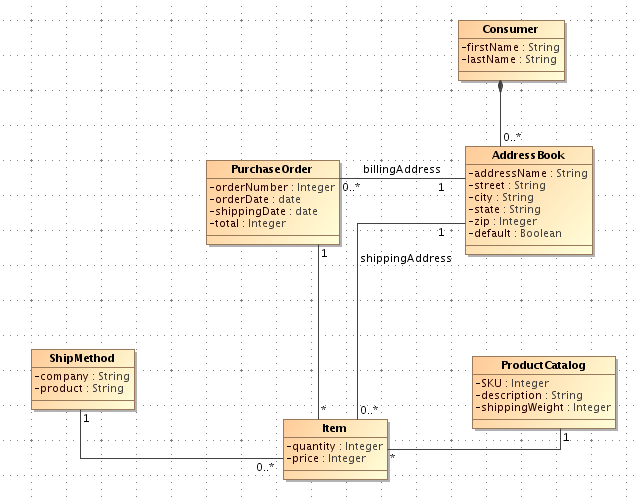
\includegraphics[width=140mm]{a.png}

\pagebreak

2)

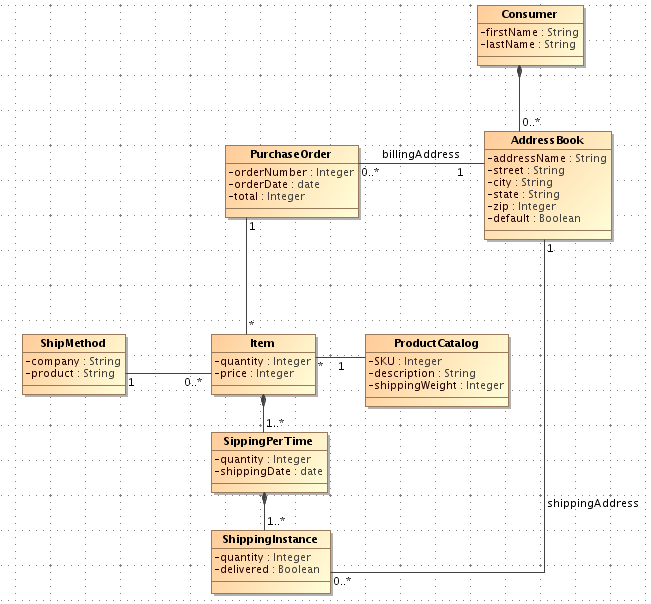
\includegraphics[width=140mm]{b.png}

\end{document}
